\ifdefined\requirementspracticefragment\else
\documentclass[aspectratio=169]{beamer}

\usetheme{Boadilla}
\usefonttheme{professionalfonts}
\setbeamertemplate{navigation symbols}{}
\setbeamertemplate{itemize items}[circle]
\setbeamertemplate{enumerate items}[default]
\setbeamertemplate{headline}{}

\usepackage[utf8]{inputenc}
\usepackage[T1]{fontenc}
\usepackage{lmodern}
\usepackage{amsmath}
\usepackage{booktabs}
\usepackage{tabularx}
\usepackage{array}
\usepackage{hyperref}
\usepackage[strings]{underscore}
\usepackage{listings}
\usepackage{tikz}
\usetikzlibrary{arrows.meta,positioning,fit,calc,shapes.geometric}
\usepackage{xcolor}

\definecolor{courseblue}{HTML}{12355B}
\definecolor{coursegold}{HTML}{C98A2E}
\definecolor{courseice}{HTML}{EEF3F8}
\definecolor{coursegreen}{HTML}{2F6B4F}
\definecolor{coursegray}{HTML}{4B5563}
\definecolor{codebg}{HTML}{F7F9FC}
\definecolor{codecomment}{HTML}{5E6C84}
\definecolor{codestring}{HTML}{0B6E4F}

\setbeamercolor{palette primary}{bg=courseblue,fg=white}
\setbeamercolor{palette secondary}{bg=coursegold,fg=white}
\setbeamercolor{palette tertiary}{bg=courseblue,fg=white}
\setbeamercolor{palette quaternary}{bg=coursegold,fg=white}
\setbeamercolor{structure}{fg=courseblue}
\setbeamercolor{frametitle}{bg=courseice,fg=courseblue}
\setbeamercolor{title}{fg=courseblue}
\setbeamercolor{block title}{bg=courseblue,fg=white}
\setbeamercolor{block body}{bg=courseice,fg=black}
\setbeamercolor{normal text}{fg=black,bg=white}
\setbeamercolor{alerted text}{fg=coursegold}

\setbeamerfont{footline}{size=\scriptsize}

\setbeamertemplate{footline}{
  \leavevmode
  \hbox{
    \begin{beamercolorbox}[wd=.33\paperwidth,ht=2.8ex,dp=1.2ex,leftskip=0.8em]{palette primary}%
      University of Trieste
    \end{beamercolorbox}%
    \begin{beamercolorbox}[wd=.49\paperwidth,ht=2.8ex,dp=1.2ex,center]{palette tertiary}%
      \coursename{} \textbar{} \coursecode
    \end{beamercolorbox}%
    \begin{beamercolorbox}[wd=.18\paperwidth,ht=2.8ex,dp=1.2ex,rightskip=0.8em plus1fil]{palette secondary}%
      \insertframenumber{} / \inserttotalframenumber
    \end{beamercolorbox}%
  }
}

\hypersetup{
  colorlinks=true,
  linkcolor=courseblue,
  urlcolor=coursegreen
}

\lstdefinestyle{coursepython}{
  language=Python,
  basicstyle=\ttfamily\footnotesize,
  keywordstyle=\color{courseblue}\bfseries,
  commentstyle=\color{codecomment}\itshape,
  stringstyle=\color{codestring},
  showstringspaces=false,
  columns=fullflexible,
  keepspaces=true,
  frame=single,
  framerule=0.6pt,
  rulecolor=\color{courseblue},
  backgroundcolor=\color{codebg},
  xleftmargin=0.4em,
  xrightmargin=0.4em,
  aboveskip=0.4em,
  belowskip=0.2em
}

\newcommand{\coursename}{Data-driven Systems Engineering}
\newcommand{\coursecode}{440MI / 305SM}
\newcommand{\coursefooter}{}

\newcommand{\learninggoals}[1]{
  \begin{block}{Learning goals}
  #1
  \end{block}
}

\newcommand{\repoactivity}[1]{
  \begin{block}{Repo activity}
  #1
  \end{block}
}

\newcommand{\readinglist}[1]{
  \begin{block}{Papers and materials}
  {\footnotesize #1}
  \end{block}
}

\newcommand{\coursecontextframe}[5]{
  \begin{frame}{Course Map and Running Cases}
  \centering
  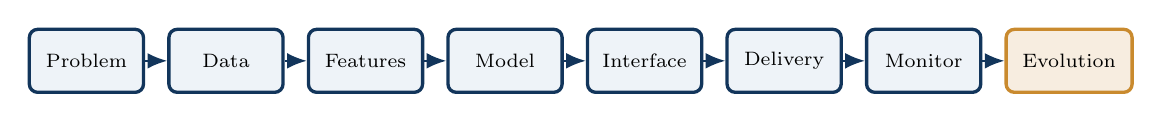
\begin{tikzpicture}[node distance=0.28cm]
  \node[flowbox, minimum width=1.45cm, minimum height=0.8cm] (problem) {\scriptsize Problem};
  \node[flowbox, minimum width=1.45cm, minimum height=0.8cm, right=of problem] (data) {\scriptsize Data};
  \node[flowbox, minimum width=1.45cm, minimum height=0.8cm, right=of data] (features) {\scriptsize Features};
  \node[flowbox, minimum width=1.45cm, minimum height=0.8cm, right=of features] (model) {\scriptsize Model};
  \node[flowbox, minimum width=1.45cm, minimum height=0.8cm, right=of model] (interface) {\scriptsize Interface};
  \node[flowbox, minimum width=1.45cm, minimum height=0.8cm, right=of interface] (delivery) {\scriptsize Delivery};
  \node[flowbox, minimum width=1.45cm, minimum height=0.8cm, right=of delivery] (monitor) {\scriptsize Monitor};
  \node[accentbox, minimum width=1.6cm, minimum height=0.8cm, right=of monitor] (evolution) {\scriptsize Evolution};
  \foreach \a/\b in {problem/data,data/features,features/model,model/interface,interface/delivery,delivery/monitor,monitor/evolution} {
    \draw[arrow] (\a) -- (\b);
  }
  \end{tikzpicture}

  \vspace{0.5em}
  \begin{block}{Today in the course}
  \textbf{Focus:} #1

  \textbf{Bridge:} #2
  \end{block}

  \begin{columns}[T]
  \column{0.48\textwidth}
  \begin{block}{Fraud case}
  {\footnotesize #3}
  \end{block}
  \column{0.48\textwidth}
  \begin{block}{Pasteurization case}
  {\footnotesize #4}
  \end{block}
  \end{columns}

  \vspace{0.3em}
  {\footnotesize \textbf{Course thread:} #5}
  \coursefooter
  \end{frame}
}

\newcommand{\classclosingframe}[4]{
  \begin{frame}{From This Class to the Next}
  \begin{block}{What stays with us}
  #1
  \end{block}

  \begin{columns}[T]
  \column{0.48\textwidth}
  \begin{block}{Project use}
  {\footnotesize #2}
  \end{block}
  \column{0.48\textwidth}
  \begin{block}{Next connection}
  {\footnotesize #3}
  \end{block}
  \end{columns}

  \vspace{0.3em}
  {\footnotesize \textbf{Course thread:} #4}
  \coursefooter
  \end{frame}
}

\tikzset{
  flowbox/.style={
    rounded corners=3pt,
    draw=courseblue,
    fill=courseice,
    very thick,
    minimum width=2.2cm,
    minimum height=0.9cm,
    align=center,
    font=\small
  },
  accentbox/.style={
    rounded corners=3pt,
    draw=coursegold,
    fill=coursegold!15,
    very thick,
    minimum width=2.2cm,
    minimum height=0.9cm,
    align=center,
    font=\small
  },
  arrow/.style={
    -{Latex[length=2.5mm,width=2mm]},
    thick,
    draw=courseblue
  }
}

\title{Class 22: Requirements Engineering in Practice}
\author{\coursename}
\date{}
\begin{document}
\frame{\titlepage \coursefooter}
\fi

\section{4. Put it into practice}
\begin{frame}[c]
\centering
{\usebeamerfont{title}\usebeamercolor[fg]{title}4. Put it into practice\par}
\vspace{1em}
Apply the same principles to a hypothetical library assistant.
\end{frame}

\begin{frame}{Mini-workshop: a hypothetical library assistant}
\begin{block}{Scenario}
A library wants an ML assistant that suggests books from a reader	extquotesingle s stated interests. A librarian reviews the suggestions before sharing them.
\end{block}
\begin{itemize}
\item Work in pairs for 15 minutes, then discuss for 5 minutes.
\item Use this fictional scenario; no code or dataset is needed.
\item Any invented threshold must be marked as an assumption to validate.
\end{itemize}
\coursefooter
\end{frame}

\begin{frame}{First, clarify the need (3 minutes)}
\begin{itemize}
\item Who uses the suggestions, and what decision do they make?
\item What makes a suggestion useful to a reader?
\item What happens if no suitable book is available?
\item What information about readers may be retained?
\end{itemize}\begin{block}{Output}
Write two questions for the librarian and two explicit assumptions. Do not invent answers and present them as confirmed requirements.
\end{block}
\coursefooter
\end{frame}

\begin{frame}{Write a small specification (7 minutes)}
\begin{itemize}
\item Write two functional requirements: name the trigger and observable result.
\item Write one non-functional requirement with clear verification conditions.
\item Write one ML quality requirement: define how relevance is judged and measured.
\item For each requirement, add an ID and a concrete acceptance check.
\end{itemize}\begin{block}{Remember}
A privacy or access rule can be testable without a numeric threshold. Use numbers when the property calls for them.
\end{block}
\coursefooter
\end{frame}

\begin{frame}{Review and negotiate (5 minutes)}
\begin{itemize}
\item Swap your specification with another pair.
\item Find one ambiguous term and propose a precise replacement.
\item Identify one conflict, such as recommendation variety versus relevance.
\item Record which goal takes priority and why.
\item Check whether another pair could run each acceptance check without asking what you meant.
\end{itemize}
\coursefooter
\end{frame}

\begin{frame}{Worked example: behavior and constraints}
\begin{block}{Functional requirement}
L1: When a librarian submits at least one interest, the system shall display up to five matching books from the available catalog; if there are no matches, it shall display ``No matching books found.
\end{block}
\begin{block}{Non-functional requirement}
L2: With 10 concurrent librarians and a catalog of 50,000 books, at least 95\% of searches shall complete within 2 seconds during a 15-minute load test.
\end{block}
\begin{itemize}
\item Check L1 with matching and empty-result fixtures. Check L2 with a load test.
\item These are proposed requirements with hypothetical conditions and targets.
\end{itemize}
\coursefooter
\end{frame}

\begin{frame}{Worked example: ML acceptance and debrief}
\begin{block}{Proposed quality requirement}
L3: On a fixed set of 100 reader profiles excluded from tuning, at least 80\% shall receive a relevant book among the top five. Two librarians shall judge relevance using an agreed rubric and resolve disagreements before scoring.
\end{block}
\begin{itemize}
\item Check L3 with a versioned evaluation report and the agreed relevance labels.
\item Discuss: does one relevant book make a list of five useful enough?
\item If few books are relevant, return fewer suggestions rather than fill all five slots.
\item Before implementation, validate the assumptions and negotiate the targets with the stakeholder.
\end{itemize}
\coursefooter
\end{frame}

\ifdefined\requirementspracticefragment\else
\end{document}
\fi
